\section{Classical Capacity of a Quantum Channel}

\begin{frame}{Definition of Classical Capacity}
    The classical capacity of a quantum channel \( \mathcal{N} \) is the maximum amount of classical information that can be transmitted per use of the channel with arbitrarily low error, as the number of channel uses goes to infinity.

    \begin{block}{Key Points}
        \begin{itemize}
            \item \( C(\mathcal{N}) \): Measures the effective transmission limit of classical data through a quantum channel.
            \item Ensures arbitrarily low error with sufficient channel uses and encoding strategies.
            \item Measured in bits per channel use.
        \end{itemize}
    \end{block}
\end{frame}


\begin{frame}{Types of Quantum Channels}
    Quantum channels often introduce errors due to interactions with the environment or system imperfections. These errors are referred to as \textbf{noise}.

    \begin{block}{Examples of Quantum Channels}
        \begin{itemize}
            \item \textbf{Depolarizing Channel:} Randomly replaces the state with a completely mixed state.
            \item \textbf{Dephasing Channel:} Reduces coherence by degrading off-diagonal terms in the density matrix.
            \item \textbf{Amplitude Damping Channel:} Models energy loss, such as photon loss in optical communication.
        \end{itemize}
    \end{block}

    \begin{center}
        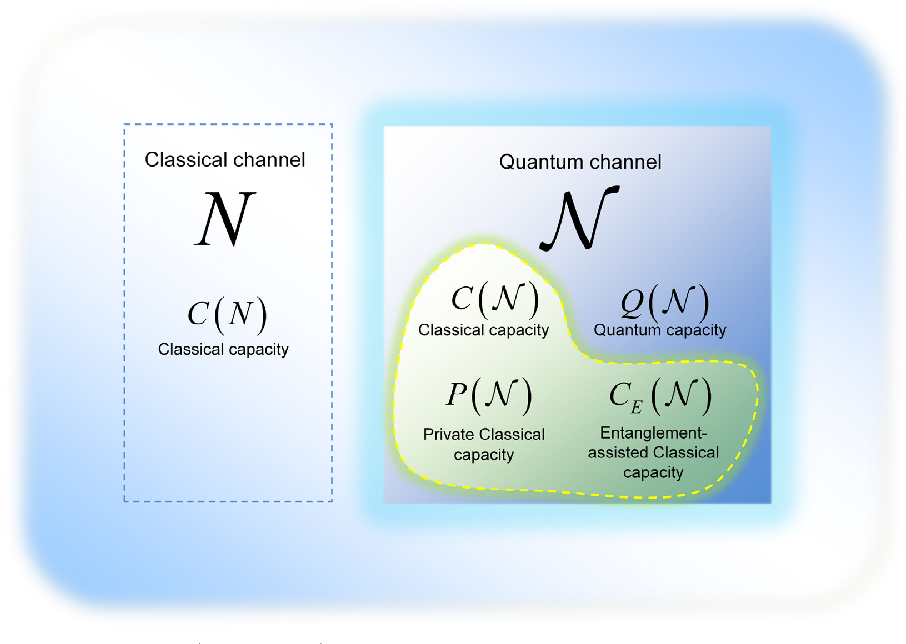
\includegraphics[width=0.5\textwidth]{figures/properties_channels.png}
    \end{center}
\end{frame}


\begin{frame}{Formula for Classical Capacity}
    The classical capacity \( C(\mathcal{N}) \) of a quantum channel \( \mathcal{N} \) is determined by the \textbf{regularized Holevo capacity}:
    \begin{equation}
        C(\mathcal{N}) = \lim_{n \to \infty} \frac{1}{n} \chi\left(\mathcal{N}^{\otimes n}\right),
    \end{equation}
    where:
    \begin{itemize}
        \item \( \mathcal{N}^{\otimes n} \): Denotes \( n \) channel uses.
        \item \( \chi \): The Holevo quantity, bounding the extractable classical information.
    \end{itemize}

    \begin{block}{Holevo Quantity}
        \[
        \chi(\mathcal{N}, \{p_i, \rho_i\}) = S\left(\sum_i p_i \mathcal{N}(\rho_i)\right) - \sum_i p_i S\left(\mathcal{N}(\rho_i)\right),
        \]
        where \( S(\rho) = -\text{Tr}(\rho \log \rho) \) is the von Neumann entropy.
    \end{block}

    \begin{center}
        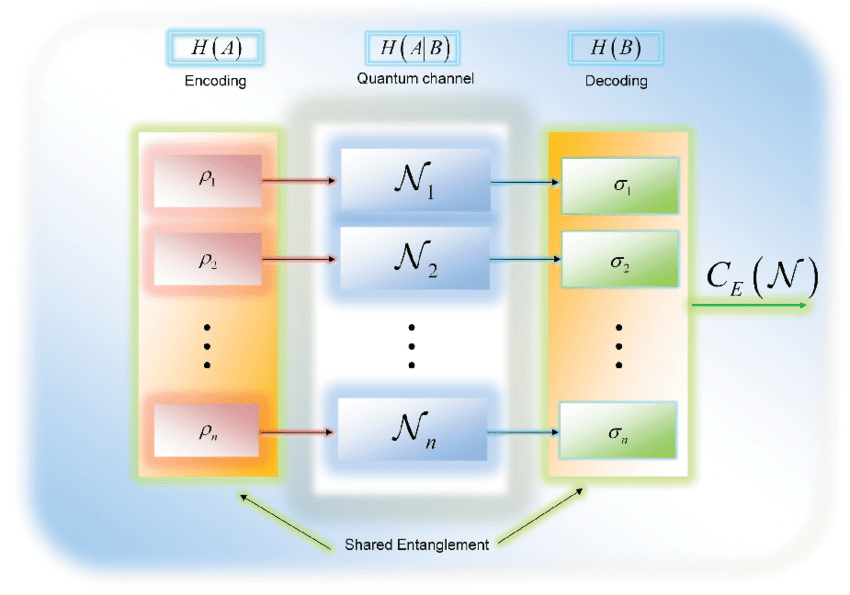
\includegraphics[width=0.65\textwidth]{figures/classical_cap.png}
    \end{center}
\end{frame}
